\documentclass[fleqn,leqno]{article}
\usepackage{amsmath, amssymb,amsfonts}
\usepackage{physics}
\usepackage{graphicx}
\usepackage{wrapfig}
\usepackage{CTEX}
\usepackage[rightcaption]{sidecap}
\usepackage[mathscr]{euscript} 
\graphicspath{ {./image/} }\makeatletter
\newif\ifkp@upRm% is used in the .fd-file of jkp
\DeclareSymbolFont{Letters}{OML}{jkp}{m}{n}
\DeclareMathSymbol{\uppartial}{\mathord}{Letters}{128}
\@addtoreset{equation}{section}
\makeatother
\renewcommand{\theequation}%
{\thesection.\arabic{equation}}
\graphicspath{{D:/code/C--practice/image/}}
\begin{document}
	\section{First section}
	\begin{equation*}
		\begin{split}
			&H_(q)=\sum_{i=1}^{D} \frac{\partial L}{\partial q} \dot{q} - L(q,t) \\
			&\frac{d}{dt} \frac{\partial L}{\partial x}-\frac{\partial L}{\partial x}=0\\
			&\frac{d}{dt} \frac{\partial L}{\partial y}-\frac{\partial L(q,\dot{q},t)}{\partial y}=0\\
			&\frac{d}{dt} \frac{\partial L(q,\dot{q},t)}{\partial q_{\beta}}-\frac{\partial L(q,\dot{q},t)}{\partial q_{\beta}} = \sum_{\alpha}\lambda_{\alpha}\frac{\partial G_{\alpha}(q,t)}{\partial q_{\beta}}\\
			&\frac{dH}{dt} = -\frac{\partial L}{\partial t}=\frac{\partial H}{\partial t}\\
			&-\frac{\partial H(q,p,t)}{\partial q_{\alpha}}=\dot{p_{\alpha}}\\
			&\frac{\partial H(q,p,t)}{\partial p_{\beta}} = \dot{q_{\beta}}\\
			&\dot{q}_{0}=\frac{\partial t}{\partial \beta}\\
			&\dot{q}_{k}=\frac{q_{k}'}{q_{0}'}\\
			&\int_{t_{1}}^{t_{2}} L(q_{[0]},\dot(q)_{[0]},t)dt = \int_{\beta_{1}}^{\beta_{2}}\dot{q}_{0}L(q,\frac{\dot{q}_{[0]}}{\dot{q}_{0}})d\beta\\
			&\dot{f}(q,p,t)=[f,H]+\frac{\partial f(q,p,t)}{\partial t}
		\end{split}
	\end{equation*}
	%
	\section{Second section}
	\mathindent=0mm
		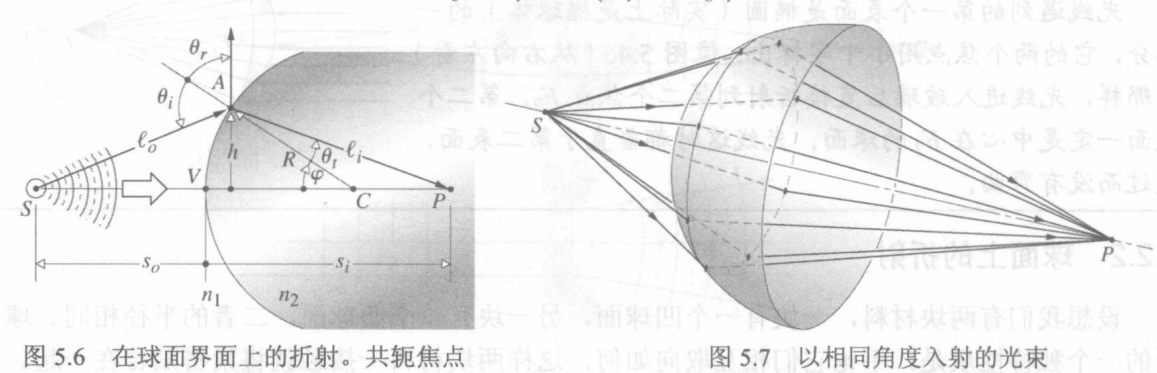
\includegraphics[width=8cm,height=4cm]{refraction.png}
		\begin{equation*}
			OPL=n_{1}(R^{2}+(s_{0}+R)^{2}-2R(s_{0}+R)cos\varphi)^{\frac{1}{2}}+n_{2}(R^{2}+(s_{1}-R)^{2}+2R(s_{1}-R)cos\varphi)^{\frac{1}{2}}
		\end{equation*}
		The power of any this lens is equal to the sum of the powers of its surfaces\\
		The telecommunications network that delivers worldwide telephone, fax, and Internet services is undergoing a quiet microphotonic revolution as it sheds its electronic elements and moves toward becoming entirely optical.\\
		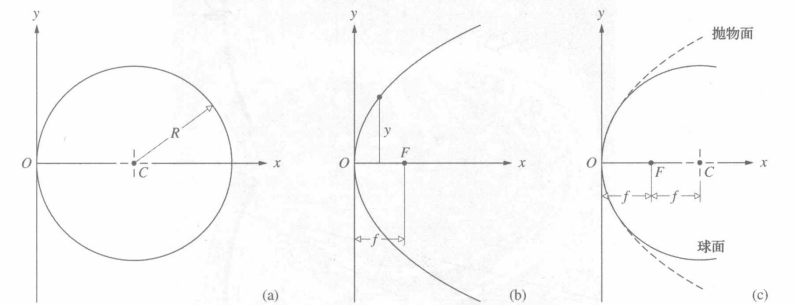
\includegraphics[width=10cm,height=4cm]{image1.png}\\
		In the paraxial region, that is, in the immediate vicinity of the central axis, these two configurations will be essentially indistinguishable.\\
		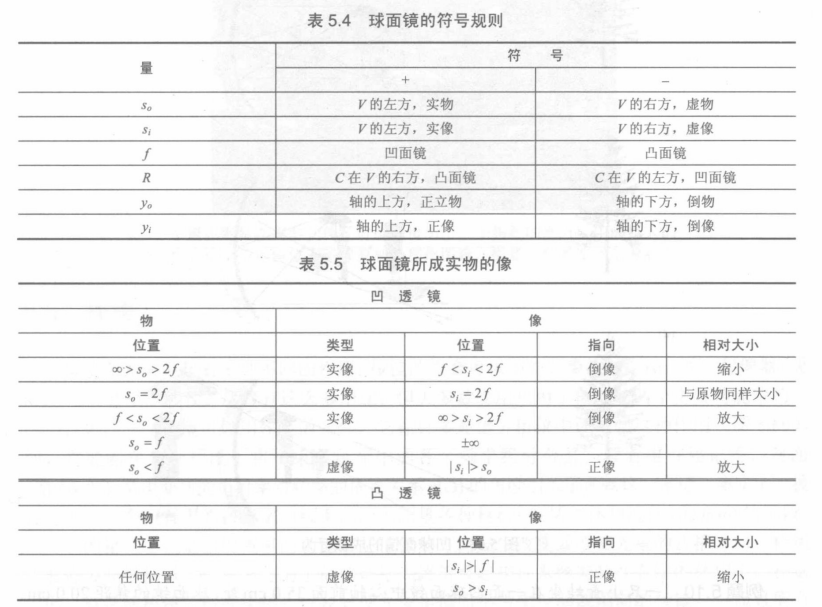
\includegraphics[width=8cm,height=8cm]{rule.png}\\
		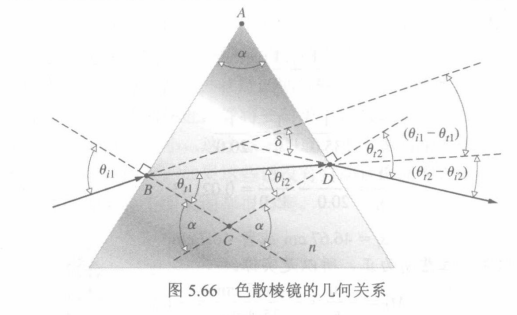
\includegraphics[width=8cm,height=6cm]{prism.png}\\
		Myopia is the condition in which parallel rays are brought to focus in front of the retina\\
		\begin{equation*}
			D_{c}=\frac{D_{\l}}{1-D_{\l}d}
		\end{equation*}
		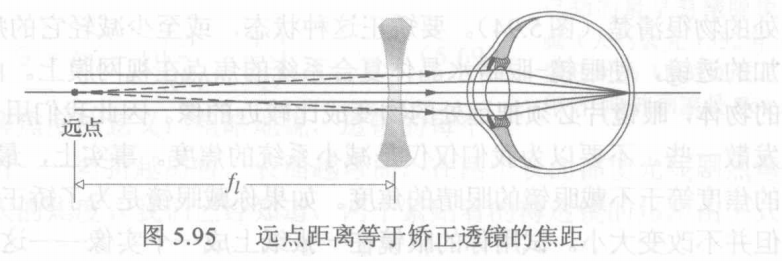
\includegraphics[width=10cm,height=4cm]{far point.png}\\
		Hyperopia (or hypermetropia) is the defect that causes the second focal point of the unaccommodated eye to lie behind the retina.\\
		\begin{equation*}
			\begin{split}
				&\tan\alpha_{a}=\alpha_{a}=\frac{y_{i}}{L}\\
				&\tan\alpha_{u}=\alpha_{u}=\frac{y_{0}}{d_{0}}\\
				&MP=\frac{\alpha_{a}}{\alpha_{u}}=\frac{y_{i}d_{0}}{y_{0}L}\\
				&MP=(1-\frac{s_{i}}{f})\frac{d_{0}}{L}\\
				&MP=\frac{d_{0}}{L}(1+D(L-\l))\\
			\end{split}
		\end{equation*}
		The Magnifying Glass\\
		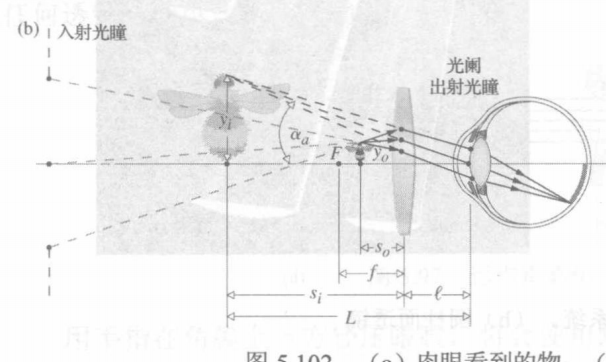
\includegraphics[width=8cm,height=6cm]{enlarge.png}\\
		A traditional single-lens reflex film camera\\
		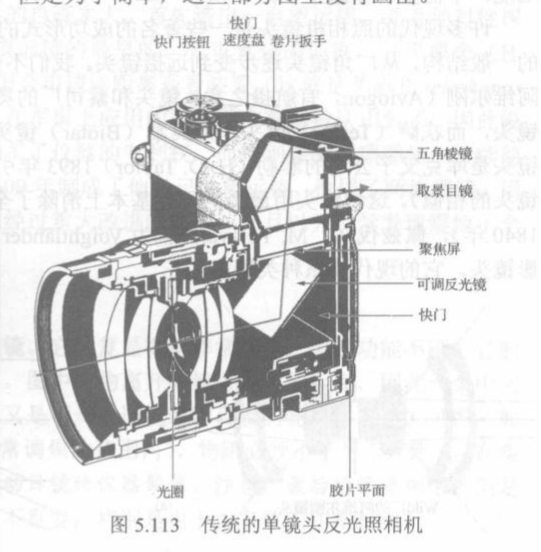
\includegraphics[width=6cm,height=6cm]{camera.png}\\
		Astronomical telescope\\
		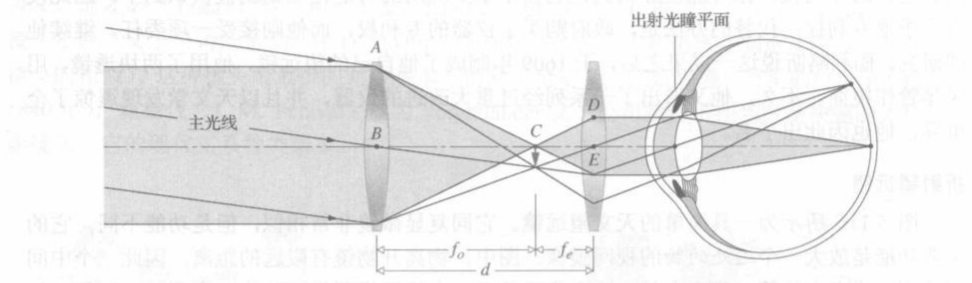
\includegraphics[width=16cm,height=6cm]{telescope.png}
		\begin{equation}
			MP=-\frac{f_{0}}{f_{e}}=\frac{D_{0}}{D_{ep}}
		\end{equation}
		The Galilean telescope
		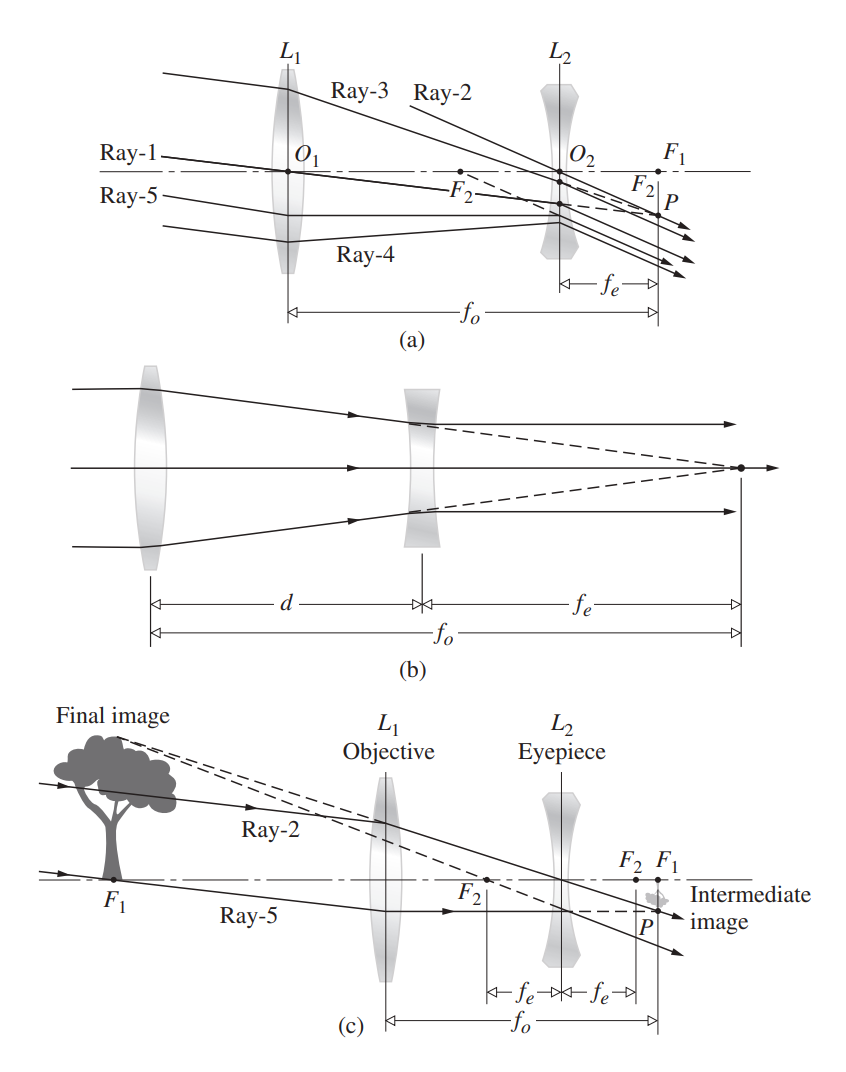
\includegraphics[width=6cm,height=8cm]{Galilean.png}
	\section{Third section}
	\mathindent=0mm
		linearly polarized light
	\begin{equation*}
			\begin{split}
				&\va{E}_{x}(z,t)=E_{0x}\cos(kz-\omega t)\\
				&\va{E}_{y}(z,t)=E_{0y}\cos(kz-\omega t+\delta)\\
				&\va{E}(z,t)=\va{i}E_{x}(z,t)+\va{j}E_{y}(z,t)\\
				&\tan{\theta}=\frac{E_{0y}}{E_{0x}}
			\end{split}
	\end{equation*}
		circularly polariazed light
		\begin{equation*}
			\begin{split}
				&\va{E}_{x}(z,t)=E_{0x}\cos(kz-\omega t)\\
				&\va{E}_{y}(z,t)=E_{0y}\cos(kz-\omega t-\frac{\pi}{2})\\
				&\va{E}(z,t)=\va{i}E_{x}(z,t)+\va{j}E_{y}(z,t)
			\end{split}
		\end{equation*}
		elliptically polarized light
		\begin{equation*}
			\begin{split}
				&\va{E}_{x}(z,t)=E_{0x}\cos(kz-\omega t)\\
				&\va{E}_{y}(z,t)=E_{0y}\cos(kz-\omega t+\varepsilon)\\
				&\left(\frac{E_{y}}{E_{0y}}\right)^{2}+\left(\frac{E_{x}}{E_{0x}}\right)^2-2\left(\frac{E_{x}}{E_{0x}}\right)\left(\frac{E_{y}}{E_{0y}}\right)\cos{\varepsilon}=\sin^2{\varepsilon}\\
				&\tan(2\alpha)=\frac{2E_{0x}E_{0y}\cos{\varepsilon}}{E_{0x}^{2}-E_{0y}^{2}}\\
				&n^2(\omega)=1+\frac{Nq^2_{e}}{\epsilon_{0}m_{e}}\sum_{j=1}^{N}\frac{f_{j}}{\omega^2_{0j}-\omega^2}
			\end{split}
		\end{equation*}
			Each individual photon exists in either spin state with equal likelihood\\
			polarizer based on 1.Dichroism 2.reflection 3.birefringence 4.scattering underlying reason:asymmetry\\
		\\	Malus Law
		\begin{equation*}
			\begin{split}
				I(\theta)=I(0)\cos^2{\theta}
			\end{split}
		\end{equation*}
	The Wire-Grid Polarizer\\
	Dichroic crystal(anisotropy)(the optics axis)\\
	Polarold J-sheet /H-sheet\\
	the principal transmittance $T_{0}$ the minor transmittance $T_{90}$
	transmittance
	\begin{equation*}
		\begin{split}
		T_{\iota}=T_{0}\cos^2{\theta}+T_{90}\sin^2{\theta}\\
		\end{split}
	\end{equation*}
	An anisotropy in the binding power will be manifest in an anisotropy in the refractive index.
	\begin{equation*}
		\begin{bmatrix}
			D_{x}\\
			D_{y}\\
			D_{z}\\
		\end{bmatrix}
	=
		\begin{bmatrix}
			\varepsilon_{xx}&\varepsilon_{xy}&\varepsilon_{xz}\\
			\varepsilon_{yx}&\varepsilon_{yy}&\varepsilon_{yz}\\
			\varepsilon_{zx}&\varepsilon_{zy}&\varepsilon_{zz}
		\end{bmatrix}
		\begin{bmatrix}
			E_{x}\\
			E_{y}\\
			E_{z}\\
		\end{bmatrix}
	\end{equation*}
	\begin{equation*}
		\begin{split}
			&n_{0}\equiv c/v_{\perp}\\
			&n_{e}\equiv c/v_{\parallel}\\
			&\Delta n=(n_{e}-n_{0})\\	
			&\delta=\frac{2\pi}{\lambda}(n_{e}-n_{0})`1\l	
		\end{split}
	\end{equation*}
	polarization angle/Brewster's angle
	\begin{equation*}
		\begin{split}
			&n_{i}\sin\theta_{p}=n_{t}\sin\theta_{t}\\
			&\theta_{p}+\theta_{t}=\frac{\pi}{2}\\
			&\tan\theta_{p}=\frac{n_{t}}{n_{i}}
		\end{split}
	\end{equation*}
	\begin{equation*}
		\begin{split}
			&r_{\bot}=-\frac{\sin(\theta_{i}-\theta_{t})}{\sin(\theta_{i}+\theta_{t})}\\
			&r_{\parallel}=+\frac{\tan(\theta_{i}-\theta_{t})}{\tan(\theta_{i}+\theta_{t})}\\
			&t_{\bot}=+\frac{2\sin\theta_{t}\cos\theta_{i}}{\sin(\theta_{i}+\theta_{t})}\\
			&t_{\parallel}=+\frac{2\sin\theta_{t}\cos\theta_{i}}{\sin(\theta_{i}+\theta_{t})\cos(\theta_{i}-\theta_{t})}
		\end{split}
	\end{equation*}
	Retarder: it advances or retards the phase of one of the two orthogonal electric fields by some desired amount.\\
	The phase shifter will always have two specified perpendicular axes, the fast and the slow.\\
	the full-wave plate    the half-wave plate
\end{document}